\documentclass{article}
\usepackage[margin=0.5in]{geometry}
\usepackage{amsmath, amssymb, hyperref, fancyhdr, graphicx}
\pagestyle{fancy}
\lhead{EE282 PA1, Artem Vasilyev \& Lingren Zhang}
\rhead{}
\begin{document}
\section{Summary}
Below is the performance summary of our current implementation obtained with GCC compiler:
\begin{table}[htbp]
\tiny
\caption{Summary}
\begin{tabular}{|r|r|r|r|r|r|r|r|r|r|r|r|}
\hline
Dim. &   MFLOPS &     Runtime & Instr completed & Total cycles & L1D misses & L2 misses & \multicolumn{1}{l|}{L1D accesses} & \multicolumn{1}{l|}{ L2 accesses} & \multicolumn{1}{l|}{L1D miss rate} & \multicolumn{1}{l|}{L2 miss rate} & \multicolumn{1}{l|}{CPI} \\ \hline
2 & 2224.86 & 0 & 39 & 17 & 0 & 0 & 18 & 0 & 0.00 & 0.00 & 0.44 \\ \hline
4 & 4339.93 & 0 & 169 & 69 & 0 & 0 & 95 & 0 & 0.00 & 0.00 & 0.41 \\ \hline
8 & 5518.53 & 0 & 1,030 & 431 & 0 & 0 & 466 & 0 & 0.00 & 0.00 & 0.42 \\ \hline
\textbf{16} & \textbf{5665.63} & \textbf{0} & \textbf{7,302} & \textbf{3,357} & \textbf{0} & \textbf{0} & \textbf{3,479} & \textbf{0} & \textbf{0.00} & \textbf{0.00} & \textbf{0.46} \\ \hline
32 & 6574.44 & 0.01 & 55,405 & 23,243 & 10 & 0 & 26,691 & 11 & 0.04 & 0.00 & 0.42 \\ \hline
64 & 6904.44 & 0.08 & 422,294 & 176,259 & 3,244 & 0 & 172,442 & 4,310 & 1.88 & 0.00 & 0.42 \\ \hline
128 & 6790.16 & 0.62 & 3,377,738 & 1,434,634 & 42,958 & 0 & 1,376,328 & 71,130 & 3.12 & 0.00 & 0.42 \\ \hline
\textbf{256} & \textbf{6475.6} & \textbf{5.18} & \textbf{27,020,868} & \textbf{12,035,110} & \textbf{513,636} & \textbf{90} & \textbf{11,011,039} & \textbf{1,204,339} & \textbf{4.66} & \textbf{0.01} & \textbf{0.45} \\ \hline
512 & 5142.12 & 52.2 & 240,684,641 & 121,874,937 & 10,649,198 & 149,363 & 86,022,844 & 19,644,528 & 12.38 & 0.76 & 0.51 \\ \hline
\textbf{1024} & \textbf{5048.63} & \textbf{425.36} & \textbf{1,902,186,269} & \textbf{994,492,897} & \textbf{80,563,811} & \textbf{2,143,165} & \textbf{681,283,251} & \textbf{158,244,880} & \textbf{11.83} & \textbf{1.35} & \textbf{0.52} \\ \hline
2048 & 4852.77 & 3540.22 & 15,217,487,071 & 8,231,334,587 & 653,247,730 & 28,407,812 & 5,455,979,061 & 1,295,043,980 & 11.97 & 2.19 & 0.54 \\ \hline
\end{tabular}
\label{}
\end{table}

For $16\times16$ we get 5665.63 MFLOPS, 0.46 CPI, 0 cache miss rate.  For $256\times256$ we get 6475.6 MFLOPS, 0.45 CPI, 4.66\% L1D cache miss rate and 0.01\% L2 cache miss rate.  For $1024\times1024$ we get 5048.63 MFLOPS, 0.52 CPI, 11.83\% L1D cache miss rate and 1.35\% L2 cache miss rate.  Below is a plot of improvements achieved via various optimizations:

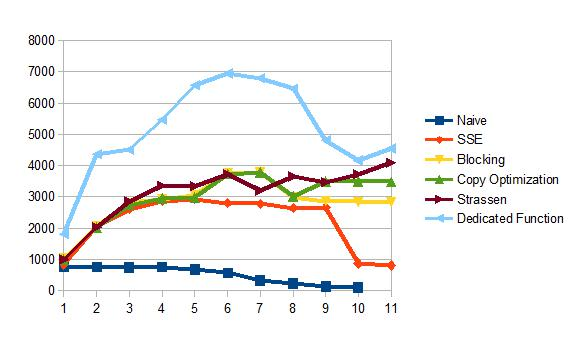
\includegraphics[scale = 0.8]{Performance.jpg}


\section{Optimizations Attempted}
\subsection{Naive Implementation}
\begin{table}[htbp]
\tiny
\caption{Naive Implementation}
\begin{tabular}{|r|r|r|r|r|r|r|r|r|r|r|r|}
\hline
Dim. &   MFLOPS &     Runtime & Instr completed & Total cycles & L1D misses & L2 misses & \multicolumn{1}{l|}{L1D accesses} & \multicolumn{1}{l|}{ L2 accesses} & \multicolumn{1}{l|}{L1D miss rate} & \multicolumn{1}{l|}{L2 miss rate} & \multicolumn{1}{l|}{CPI} \\ \hline
2 & 765.21 & 0 & 133 & 49 & 0 & 0 & 48 & 0 & 0 & 0 & 0.37 \\ \hline
4 & 754.63 & 0 & 681 & 394 & 0 & 0 & 349 & 0 & 0 & 0 & 0.58 \\ \hline
8 & 747.73 & 0 & 4,633 & 3,181 & 0 & 0 & 2,710 & 0 & 0 & 0 & 0.69 \\ \hline
16 & 755.32 & 0.01 & 34,713 & 25,189 & 0 & 0 & 20,948 & 0 & 0 & 0 & 0.73 \\ \hline
32 & 681.6 & 0.1 & 269,593 & 223,389 & 27 & 0 & 156,639 & 377 & 0.02 & 0 & 0.83 \\ \hline
64 & 574.58 & 0.91 & 2,126,362 & 2,119,160 & 24,526 & 0 & 1,297,288 & 33,260 & 1.89 & 0 & 1 \\ \hline
128 & 331.33 & 12.66 & 16,892,960 & 29,443,156 & 2,427,569 & 8 & 10,991,681 & 2,434,546 & 22.09 & 0 & 1.74 \\ \hline
256 & 227.58 & 147.44 & 134,678,638 & 343,480,488 & 24,922,029 & 2,694 & 92,193,892 & 24,950,234 & 27.03 & 0.01 & 2.55 \\ \hline
512 & 140.98 & 1904.12 & 1,075,581,786 & 4,430,396,405 & 266,979,850 & 116,361 & 932,074,078 & 255,066,744 & 28.64 & 0.05 & 4.12 \\ \hline
1024 & 100.33 & 21405.34 & 8,597,289,381 & 49,697,805,160 & 1,848,707,670 & 483,279,194 & 7,499,536,772 & 2,140,510,921 & 24.65 & 22.58 & 5.78 \\ \hline
2048 & NA & NA & NA & NA & NA & NA & NA & NA & NA & NA & NA \\ \hline
\end{tabular}
\label{}
\end{table}

\subsection{SSE2}
SSE are 128-bit vector instructions which take advantage of the data level parallelism and can do two double precision math operations instead of one.  The operation performed on two pairs has to be the same (two multiplications or two additions etc). We expect to get about 2$\times$ performance increase with this. And after implementation there is a jump for all matrices except $2\times 2$ which goes from 770 MOPS to 830 MOPS. The desrepancy for the $2\times2$ matrix is because of the large \% of overhead instructions compared to those for the bigger matrixes.
\url{http://en.wikipedia.org/wiki/SSE2}

In addition, we expect to see fewer L1 and L2 cache misses due to the fact that in the SSE2 implementation we access both A and B matrix in row major order which aligns with the way they are stored, we expect cache misses to reduce to about $1/8$ because each cache line (64kB) holds 8 doubles.  We can verify in the table that there is a reduction in cache misses and performance improves more than $2\times$ for all matrices except $2\times2$.
\begin{table}[htbp]
\tiny
\caption{SSE2}
\begin{tabular}{|r|r|r|r|r|r|r|r|r|r|r|r|}
\hline
Dim. &   MFLOPS &     Runtime & Instr completed & Total cycles & L1D misses & L2 misses & \multicolumn{1}{l|}{L1D accesses} & \multicolumn{1}{l|}{ L2 accesses} & \multicolumn{1}{l|}{L1D miss rate} & \multicolumn{1}{l|}{L2 miss rate} & \multicolumn{1}{l|}{CPI} \\ \hline
2 & 828.69 & 0 & 100 & 45 & 0 & 0 & 27 & 0 & 0 & 0 & 0.45 \\ \hline
4 & 2054.69 & 0 & 408 & 145 & 0 & 0 & 148 & 0 & 0 & 0 & 0.36 \\ \hline
8 & 2605.96 & 0 & 2,392 & 913 & 0 & 0 & 878 & 0 & 0 & 0 & 0.38 \\ \hline
16 & 2860.74 & 0 & 16,536 & 6,681 & 0 & 0 & 6,409 & 0 & 0 & 0 & 0.4 \\ \hline
32 & 2931.63 & 0.02 & 123,160 & 51,952 & 49 & 0 & 51,208 & 77 & 0.1 & 0 & 0.42 \\ \hline
64 & 2796.38 & 0.19 & 950,808 & 435,595 & 8,252 & 0 & 408,278 & 20,820 & 2.02 & 0 & 0.46 \\ \hline
128 & 2782.1 & 1.51 & 7,472,153 & 3,492,812 & 260,189 & 1 & 3,165,435 & 671,433 & 8.22 & 0 & 0.47 \\ \hline
256 & 2640.07 & 12.71 & 59,246,623 & 29,710,225 & 2,094,890 & 1,394 & 25,635,822 & 5,264,400 & 8.17 & 0.03 & 0.5 \\ \hline
512 & 2673.49 & 100.41 & 471,863,375 & 233,233,129 & 16,851,905 & 64,861 & 203,380,807 & 42,772,351 & 8.29 & 0.15 & 0.49 \\ \hline
1024 & 867.27 & 2476.15 & 3,766,494,129 & 5,752,949,389 & 134,885,123 & 115,465,120 & 1,617,562,377 & 291,538,588 & 8.34 & 39.61 & 1.53 \\ \hline
2048 & 804.85 & 21345.33 & 30,098,347,627 & 49,512,402,723 & 1,102,078,829 & 1,078,419,568 & 12,921,475,490 & 2,209,665,130 & 8.53 & 48.8 & 1.65 \\ \hline
\end{tabular}
\label{}
\end{table}

\subsection{Blocking}
We observed in the table above that there is a large increase in L1 miss rate at $64 \times 64$ and a large increase in L2 miss rate at $1024\times1024$.  This agrees with our intuition as these are the levels where matrices no longer fit in L1/L2 cache.  Hence we implemented two-level blocking and found that having the outer block fit in L2 and inner block fit in L1 reduces cache misses effectively without introducing too much overhead (which happens when blocks are too small), we chose inner block size to be $32\times32$ and outer block size to be $256\times256$.

After implementing blocking we found that we addressed the L2 misses for $1024\times1024$ and above (reduced misses by about 99\%), however the number of L1 misses are roughly unchanged.
\begin{table}[htbp]
\tiny
\caption{Blocking}
\begin{tabular}{|r|r|r|r|r|r|r|r|r|r|r|r|}
\hline
Dim. &   MFLOPS &     Runtime & Instr completed & Total cycles & L1D misses & L2 misses & \multicolumn{1}{l|}{L1D accesses} & \multicolumn{1}{l|}{ L2 accesses} & \multicolumn{1}{l|}{L1D miss rate} & \multicolumn{1}{l|}{L2 miss rate} & \multicolumn{1}{l|}{CPI} \\ \hline
2 & 1034.24 & 0 & 108 & 36 & 0 & 0 & 37 & 0 & 0 & 0 & 0.33 \\ \hline
4 & 2051.58 & 0 & 402 & 145 & 0 & 0 & 159 & 0 & 0 & 0 & 0.36 \\ \hline
8 & 2810.96 & 0 & 2,334 & 846 & 0 & 0 & 902 & 0 & 0 & 0 & 0.36 \\ \hline
16 & 2924.69 & 0 & 16,278 & 6,503 & 0 & 0 & 6,525 & 0 & 0 & 0 & 0.4 \\ \hline
32 & 3046.51 & 0.02 & 122,118 & 49,961 & 50 & 0 & 51,224 & 62 & 0.1 & 0 & 0.41 \\ \hline
64 & 3757.69 & 0.14 & 588,455 & 325,201 & 3,170 & 0 & 321,587 & 6,910 & 0.99 & 0 & 0.55 \\ \hline
128 & 3778.83 & 1.11 & 4,707,106 & 2,579,245 & 158,412 & 0 & 2,474,710 & 308,873 & 6.4 & 0 & 0.55 \\ \hline
256 & 2995.74 & 11.2 & 37,655,771 & 25,994,903 & 2,541,172 & 1,484 & 19,767,381 & 6,088,674 & 12.86 & 0.02 & 0.69 \\ \hline
512 & 2861.05 & 93.82 & 301,255,273 & 217,682,616 & 20,510,984 & 138,611 & 158,680,725 & 47,428,252 & 12.93 & 0.29 & 0.72 \\ \hline
1024 & 2840.41 & 756.05 & 2,410,041,375 & 1,758,861,009 & 163,717,105 & 1,570,361 & 1,270,109,728 & 382,796,568 & 12.89 & 0.41 & 0.73 \\ \hline
2048 & 2832.92 & 6064.38 & 19,280,328,546 & 14,091,166,204 & 1,310,251,939 & 12,907,808 & 10,162,617,221 & 3,068,467,646 & 12.89 & 0.42 & 0.73 \\ \hline
\end{tabular}
\label{}
\end{table}

\subsection{Copy Optimization}
We realized that there are both capacity misses and conflict misses in L1 cache, and blocking only addresses capacity misses.  Even though we make sure that there is enough space in L1 for each inner block, block entries in the same column evict each other when the matrix is large.  The solution is to perform copy optimization for matrix B (when matrix size is large).  In particular, we store matrix B in row major order by inner block to make sure that each inner block has consecutive addresses in the memory.

After implementing copy optimization for $512\times512$ and above, we reduced L1 misses by about 90\%, we see in the table that $256\times256$ can potentially benefit from copy optimization as well.

\begin{table}[htbp]
\tiny
\caption{Copy Optimization}
\begin{tabular}{|r|r|r|r|r|r|r|r|r|r|r|r|}
\hline
Dim. &   MFLOPS &     Runtime & Instr completed & Total cycles & L1D misses & L2 misses & \multicolumn{1}{l|}{L1D accesses} & \multicolumn{1}{l|}{ L2 accesses} & \multicolumn{1}{l|}{L1D miss rate} & \multicolumn{1}{l|}{L2 miss rate} & \multicolumn{1}{l|}{CPI} \\ \hline
2 & 999.68 & 0 & 112 & 37 & 0 & 0 & 37 & 0 & 0 & 0 & 0.33 \\ \hline
4 & 2017.8 & 0 & 406 & 147 & 0 & 0 & 159 & 0 & 0 & 0 & 0.36 \\ \hline
8 & 2740.57 & 0 & 2,338 & 871 & 0 & 0 & 878 & 0 & 0 & 0 & 0.37 \\ \hline
16 & 2950.66 & 0 & 16,282 & 6,486 & 0 & 0 & 6,437 & 0 & 0 & 0 & 0.4 \\ \hline
32 & 2983.02 & 0.02 & 122,122 & 51,222 & 33 & 0 & 51,212 & 79 & 0.06 & 0 & 0.42 \\ \hline
64 & 3726.41 & 0.14 & 588,459 & 326,448 & 3,140 & 0 & 322,275 & 6,920 & 0.97 & 0 & 0.55 \\ \hline
128 & 3778.83 & 1.11 & 4,707,110 & 2,578,561 & 157,631 & 0 & 2,483,860 & 309,927 & 6.35 & 0 & 0.55 \\ \hline
256 & 3007.68 & 11.16 & 37,655,775 & 25,905,635 & 2,544,461 & 234 & 19,844,811 & 6,073,872 & 12.82 & 0 & 0.69 \\ \hline
512 & 3489.44 & 76.93 & 301,315,987 & 179,597,106 & 1,852,325 & 170,039 & 167,058,409 & 3,770,847 & 1.11 & 4.51 & 0.6 \\ \hline
1024 & 3485.96 & 616.04 & 2,409,758,825 & 1,431,398,212 & 14,656,464 & 1,418,949 & 1,333,392,370 & 29,912,050 & 1.1 & 4.74 & 0.59 \\ \hline
2048 & 3483.13 & 4932.31 & 19,275,004,836 & 11,445,462,655 & 116,738,832 & 11,621,088 & 10,656,559,365 & 235,923,029 & 1.1 & 4.93 & 0.59 \\ \hline
\end{tabular}
\label{}
\end{table}

\subsection{Strassen Algorithm}
This is recursive algorithm with work on block matrices and trades matrix multiplication for additions and subtractions.  
In block form a N$\times$N matrix multiplication can be represented by 8 matrix multiplications and 4 additions where every matrix is N/2$\times$N/2. Strassen algorithm does the same operation with 7 multiplications and 18 additions/subtractions.  It is more efficient for large matrix sizes because there are $O(N^3)$ multiplications and $O(N^2)$ additions.  Empirically,  somewhere around N=100 Strassen method becomes better. \url{http://en.wikipedia.org/wiki/Strassen_algorithm}

Strassen algorithm does blocking and copy optimization intrinsically, which is desirable.  As a result it can be built directly on top of SSE2.
After implementation we saw a jump from 800 MOPS to 4000 MOPS for $2048\times2048$ (compared to SSE2).  There is also significant increase in MOPS compared to results with blocking and copy optimization for large matrices.

\begin{table}[htbp]
\tiny
\caption{Strassen Algorithm}
\begin{tabular}{|r|r|r|r|r|r|r|r|r|r|r|r|}
\hline
Dim. &   MFLOPS &     Runtime & Instr completed & Total cycles & L1D misses & L2 misses & \multicolumn{1}{l|}{L1D accesses} & \multicolumn{1}{l|}{ L2 accesses} & \multicolumn{1}{l|}{L1D miss rate} & \multicolumn{1}{l|}{L2 miss rate} & \multicolumn{1}{l|}{CPI} \\ \hline
2 & 1006.24 & 0 & 112 & 37 & 0 & 0 & 37 & 0 & 0 & 0 & 0.33 \\ \hline
4 & 2028.61 & 0 & 406 & 147 & 0 & 0 & 159 & 0 & 0 & 0 & 0.36 \\ \hline
8 & 2854.2 & 0 & 2,338 & 837 & 0 & 0 & 904 & 0 & 0 & 0 & 0.36 \\ \hline
16 & 3353.74 & 0 & 16,282 & 5,675 & 0 & 0 & 6,434 & 0 & 0 & 0 & 0.35 \\ \hline
32 & 3341.01 & 0.02 & 122,122 & 45,672 & 52 & 0 & 51,353 & 91 & 0.1 & 0 & 0.37 \\ \hline
64 & 3725.36 & 0.14 & 588,189 & 326,914 & 3,251 & 0 & 323,153 & 6,835 & 1.01 & 0 & 0.56 \\ \hline
128 & 3209.63 & 1.31 & 5,281,353 & 3,041,091 & 112,973 & 8 & 2,516,693 & 261,675 & 4.49 & 0 & 0.58 \\ \hline
256 & 3648.82 & 9.2 & 38,238,143 & 23,242,620 & 908,753 & 12,147 & 18,139,077 & 2,108,277 & 5.01 & 0.58 & 0.61 \\ \hline
512 & 3470.93 & 77.34 & 272,671,869 & 180,868,308 & 6,918,552 & 471,378 & 129,107,749 & 15,885,967 & 5.36 & 2.97 & 0.66 \\ \hline
1024 & 3728.04 & 576.04 & 1,928,648,786 & 1,337,214,224 & 50,241,481 & 5,095,813 & 911,634,956 & 115,407,390 & 5.51 & 4.42 & 0.69 \\ \hline
2048 & 4086.3 & 4204.26 & 13,580,226,806 & 9,757,932,695 & 358,655,023 & 47,004,377 & 6,409,543,523 & 813,640,172 & 5.6 & 5.78 & 0.72 \\ \hline
\end{tabular}
\label{}
\end{table}

\subsection{Dedicated Functions}
We wrote the generic function that can do any size using all the trick we could think of: blocking, loop reodering, SSE etc. but the performance still was not enough. Based on the successful experiment using dedicated functions for small N (2-32) we created similar functions for all other size. Dedicated function have an advantage that all the loop boundaries are fixed as well as arguments in pointer manipulations. This allows the compiler to do more aggresive optimizations (like unroll some loops and reorder operations) and reduces the total instruction count.  For small N  the general function can be simplified - the 3 outer loops are not needed and we could reuse data in registers from previous loop iterations  - that mean less loads and stores.

The results of this optimization varied, but on average we saw about 20\% improvement. The best case was $2\times2$ kernel where we went from 103 to 51 instructions and by reusing registers to about 40 (number varies from compile to compile) and over 2 times performance increase, for 64x64 the instruction count was reduced from 483K to 422K and performance went up by 25\%.

\begin{table}[htbp]
\tiny
\caption{Dedicated Functions}
\begin{tabular}{|r|r|r|r|r|r|r|r|r|r|r|r|}
\hline
Dim. &   MFLOPS &     Runtime & Instr completed & Total cycles & L1D misses & L2 misses & \multicolumn{1}{l|}{L1D accesses} & \multicolumn{1}{l|}{ L2 accesses} & \multicolumn{1}{l|}{L1D miss rate} & \multicolumn{1}{l|}{L2 miss rate} & \multicolumn{1}{l|}{CPI} \\ \hline
2 & 1805.83 & 0 & 44 & 21 & 0 & 0 & 22 & 0 & 0 & 0 & 0.48 \\ \hline
4 & 4366.92 & 0 & 174 & 68 & 0 & 0 & 99 & 0 & 0 & 0 & 0.39 \\ \hline
8 & 4503.28 & 0 & 1,150 & 528 & 0 & 0 & 623 & 0 & 0 & 0 & 0.46 \\ \hline
16 & 5459.13 & 0 & 8,999 & 3,499 & 0 & 0 & 4,507 & 0 & 0 & 0 & 0.39 \\ \hline
32 & 6572.47 & 0.01 & 55,409 & 23,259 & 12 & 0 & 26,694 & 18 & 0.04 & 0 & 0.42 \\ \hline
64 & 6940.07 & 0.08 & 422,298 & 176,214 & 3,249 & 0 & 172,443 & 4,267 & 1.88 & 0 & 0.42 \\ \hline
128 & 6794.34 & 0.62 & 3,377,742 & 1,434,701 & 43,028 & 0 & 1,376,330 & 70,856 & 3.13 & 0 & 0.42 \\ \hline
256 & 6449.8 & 5.2 & 27,020,872 & 12,040,422 & 515,048 & 225 & 11,011,004 & 1,206,328 & 4.68 & 0.02 & 0.45 \\ \hline
512 & 4812.29 & 55.78 & 247,304,246 & 129,315,203 & 11,542,820 & 115,943 & 88,459,296 & 20,492,626 & 13.05 & 0.57 & 0.52 \\ \hline
1024 & 4161.53 & 516.03 & 1,670,373,328 & 1,192,039,842 & 44,462,792 & 5,039,958 & 833,376,675 & 102,891,767 & 5.34 & 4.9 & 0.71 \\ \hline
2048 & 4554.29 & 3772.24 & 11,772,294,887 & 8,773,104,515 & 319,598,020 & 46,714,355 & 5,884,662,574 & 731,447,323 & 5.43 & 6.39 & 0.75 \\ \hline
\end{tabular}
\label{}
\end{table}

\subsection{Loop Unrolling/ Blocking}
Loop unrolling is similar to blocking but the reason we call in different is that it had a different goal. Blocking was aimed to reduce the miss rate to the cache while unrolling to reduce the number or operations espcially load/store.

The optimization was started to increase 32x32 performance because there was a big fall from 16 to 32 and the reason initially was unclear - the cache miss rate was pretty low. After examining the code we realize that we pulled A and then computer sumterms of every C meaning that we load/strore C every time that A changes and if we unroll the loop and read 2-4-8 different A values, we can compute 2-4-8 componets of each C and cut the number of load/store opetation and math operation (C is accumulator and by working on 2-4-8 we can implement a tree adder structure instead of array like). After implementing this we saw total instructions drop from 73485 to 55808 and load/store from 19980/18503 to 21516/4103 which gave a performance increace of 60\% (4070MFLOPS vs 6515)
\begin{table}[htbp]
\tiny
\caption{Loop Unrolling/Blocking}
\begin{tabular}{|r|r|r|r|r|r|r|r|r|r|r|r|}
\hline
Dim. &   MFLOPS &     Runtime & Instr completed & Total cycles & L1D misses & L2 misses & \multicolumn{1}{l|}{L1D accesses} & \multicolumn{1}{l|}{ L2 accesses} & \multicolumn{1}{l|}{L1D miss rate} & \multicolumn{1}{l|}{L2 miss rate} & \multicolumn{1}{l|}{CPI} \\ \hline
2 & 2224.86 & 0 & 39 & 17 & 0 & 0 & 18 & 0 & 0.00 & 0.00 & 0.44 \\ \hline
4 & 4339.93 & 0 & 169 & 69 & 0 & 0 & 95 & 0 & 0.00 & 0.00 & 0.41 \\ \hline
8 & 5518.53 & 0 & 1,030 & 431 & 0 & 0 & 466 & 0 & 0.00 & 0.00 & 0.42 \\ \hline
\textbf{16} & \textbf{5665.63} & \textbf{0} & \textbf{7,302} & \textbf{3,357} & \textbf{0} & \textbf{0} & \textbf{3,479} & \textbf{0} & \textbf{0.00} & \textbf{0.00} & \textbf{0.46} \\ \hline
32 & 6574.44 & 0.01 & 55,405 & 23,243 & 10 & 0 & 26,691 & 11 & 0.04 & 0.00 & 0.42 \\ \hline
64 & 6904.44 & 0.08 & 422,294 & 176,259 & 3,244 & 0 & 172,442 & 4,310 & 1.88 & 0.00 & 0.42 \\ \hline
128 & 6790.16 & 0.62 & 3,377,738 & 1,434,634 & 42,958 & 0 & 1,376,328 & 71,130 & 3.12 & 0.00 & 0.42 \\ \hline
\textbf{256} & \textbf{6475.6} & \textbf{5.18} & \textbf{27,020,868} & \textbf{12,035,110} & \textbf{513,636} & \textbf{90} & \textbf{11,011,039} & \textbf{1,204,339} & \textbf{4.66} & \textbf{0.01} & \textbf{0.45} \\ \hline
512 & 5142.12 & 52.2 & 240,684,641 & 121,874,937 & 10,649,198 & 149,363 & 86,022,844 & 19,644,528 & 12.38 & 0.76 & 0.51 \\ \hline
\textbf{1024} & \textbf{5048.63} & \textbf{425.36} & \textbf{1,902,186,269} & \textbf{994,492,897} & \textbf{80,563,811} & \textbf{2,143,165} & \textbf{681,283,251} & \textbf{158,244,880} & \textbf{11.83} & \textbf{1.35} & \textbf{0.52} \\ \hline
2048 & 4852.77 & 3540.22 & 15,217,487,071 & 8,231,334,587 & 653,247,730 & 28,407,812 & 5,455,979,061 & 1,295,043,980 & 11.97 & 2.19 & 0.54 \\ \hline
\end{tabular}
\label{}
\end{table}

\subsection{Compiler Flags}
For all the optimizations that we have implemented above, we used GCC compiler.  ICC gives worse results except $2 \times 2$ case which is better due to fewer instructions.

We've also tried -funroll-loop flag to unroll loops and -ftree-vectorize to do SSE2 automatically.  However, neither flag seems to make a lot of difference and we end up implementing both unrolling and SSE2 manually.

\subsection{Observation}
There were a number of artifacts we observed. Performance numbers vary noticably  from compile to compile and depending on whose account was used.  SSE2 \_mm\_set is slower that load + unpack. For some sizes ICC worked better that GCC. We also saw results missmatch with ICC but not GCC and it was different on cluster vs drink or our local machine.

\end{document}
